%\documentclass[a4paper,10pt]{report}
\documentclass[a4paper,12pt]{article}
\usepackage[utf8]{inputenc}

%----------------------------------------------------------------------------------------
%	PACKAGES AND OTHER DOCUMENT CONFIGURATIONS
%----------------------------------------------------------------------------------------

%\documentclass[twoside]{article}
%\documentclass[a4paper,12pt]{article}

%\usepackage{lipsum} % Package to generate dummy text throughout this template
\usepackage{mathtools} % package fixes some amsmath quirks and adds some useful settings, symbols, and environments to amsmath
\usepackage[sc]{mathpazo} % Use the Palatino font
\usepackage[T1]{fontenc} % Use 8-bit encoding that has 256 glyphs
\linespread{1.05} % Line spacing - Palatino needs more space between lines
\usepackage{microtype} % Slightly tweak font spacing for aesthetics

\usepackage[hmarginratio=1:1,top=32mm,columnsep=20pt]{geometry} % Document margins
\usepackage{multicol} % Used for the two-column layout of the document
\usepackage[hang, small,labelfont=bf,up,textfont=it,up]{caption} % Custom captions under/above floats in tables or figures
\usepackage{booktabs} % Horizontal rules in tables
\usepackage{float} % Required for tables and figures in the multi-column environment - they need to be placed in specific locations with the [H] (e.g. \begin{table}[H])
\usepackage{hyperref} % For hyperlinks in the PDF

\usepackage{lettrine} % The lettrine is the first enlarged letter at the beginning of the text
\usepackage{paralist} % Used for the compactitem environment which makes bullet points with less space between them
\usepackage{url}
\usepackage{cite}
%\usepackage[numbers,sort&compress]{natbib}
%\usepackage[style=numeric]{biblatex}
%\addbibresource{thomastsai.bib}
%\bibliographystyle{ieeetr}

\usepackage{abstract} % Allows abstract customization
\renewcommand{\abstractnamefont}{\normalfont\bfseries} % Set the "Abstract" text to bold
\renewcommand{\abstracttextfont}{\normalfont\small\itshape} % Set the abstract itself to small italic text

%http://en.wikibooks.org/wiki/LaTeX/Floats,_Figures_and_Captions
\usepackage{graphicx}
\usepackage{subcaption}
\graphicspath{ {dft/} }
\DeclareGraphicsExtensions{.pdf,.png,.jpg}

\usepackage{titlesec} % Allows customization of titles
\renewcommand\thesection{\Roman{section}} % Roman numerals for the sections
\renewcommand\thesubsection{\Roman{subsection}} % Roman numerals for subsections
\titleformat{\section}[block]{\large\scshape\centering}{\thesection.}{1em}{} % Change the look of the section titles
\titleformat{\subsection}[block]{\large}{\thesubsection.}{1em}{} % Change the look of the section titles

\usepackage{fancyhdr} % Headers and footers
\pagestyle{fancy} % All pages have headers and footers
\fancyhead{} % Blank out the default header
\fancyfoot{} % Blank out the default footer
\fancyhead[C]{Camera Sensor Applications $\bullet$ November 2014} % Custom header text $\bullet$ Vol. XXI, No. 1
\fancyfoot[RO,L]{\thepage} % Custom footer text
% Title Page
%----------------------------------------------------------------------------------------
%	TITLE SECTION
%----------------------------------------------------------------------------------------

\title{\vspace{-15mm}\fontsize{24pt}{10pt}\selectfont\textbf{Two Applications of Camera Sensors with Computer Vision}} % Article title
\author{
\large
\textsc{Thomas Tsai}\\[2mm] % Your name, \thanks{}
\normalsize www.biotrump.com \\ % Your institution
\normalsize \href{mailto:thomas@biotrump.com}{thomas@biotrump.com} % Your email address
\vspace{-5mm}
}
\date{}
\setlength{\headheight}{15pt}

%\let\myBib\thebibliography
%\let\endmyBib\endthebibliography

%\renewcommand\thebibliography[1]{\ifx\relax#1\relax\else\myBib{#1}\fi}

\begin{document}
\maketitle
%\thispagestyle{fancy} % All pages have headers and footers

%----------------------------------------------------------------------------------------
%	ABSTRACT
%----------------------------------------------------------------------------------------
\begin{abstract}
Two Applications are proposed. One is baby monitor and the other is smart glass.

\end{abstract}

\section{Baby Monitor}
\textbf{Sudden infant death syndrome (SIDS)} also known as \textbf{cot death} or \textbf{crib death} is the sudden death of an infant 
that is not predicted by medical history and remains unexplained after a thorough forensic autopsy and 
detailed death scene investigation. 
Infants are at the highest risk for SIDS during sleep. Typically the infant is found dead after having been put to bed, 
and exhibits no signs of having struggled.\cite{wiki-SIDS}\\

\begin{figure}[h]
  \centering
	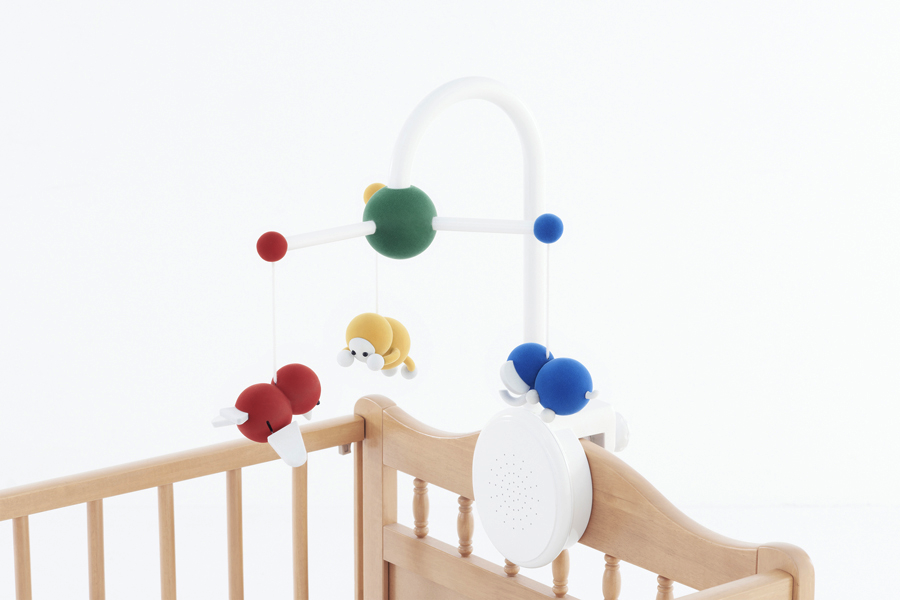
\includegraphics[width=0.7\textwidth, keepaspectratio=true]{paby-stand}
  \caption{The set of baby monitor }\cite{paby-monitor}
  \label{fig:paby-stand}
\end{figure}

\begin{figure}[h]
  \centering
	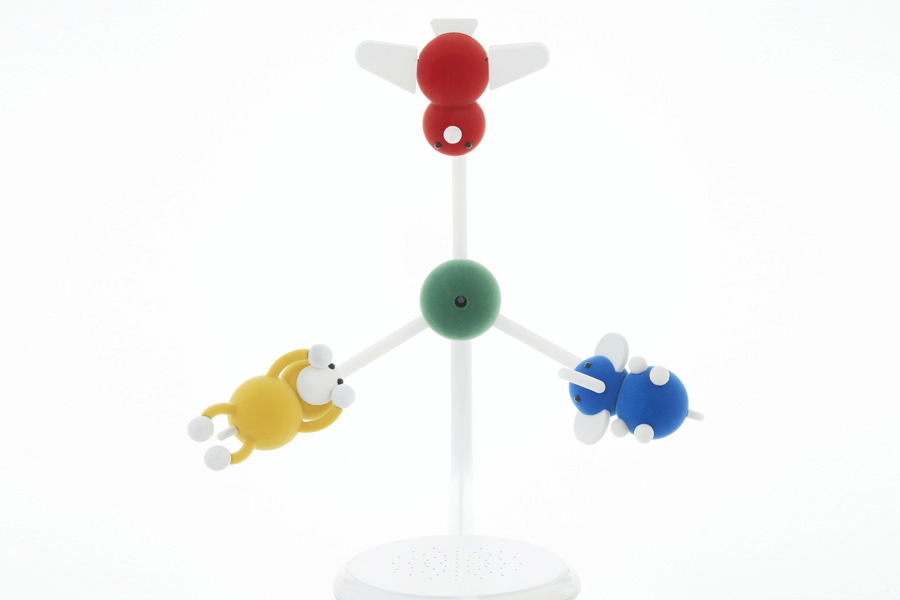
\includegraphics[width=0.7\textwidth, keepaspectratio=true]{paby-camera}
  \caption{The camera of the baby monitor}\cite{paby-monitor}
  \label{fig:paby-camera}
\end{figure}

\begin{figure}[h]
  \centering
	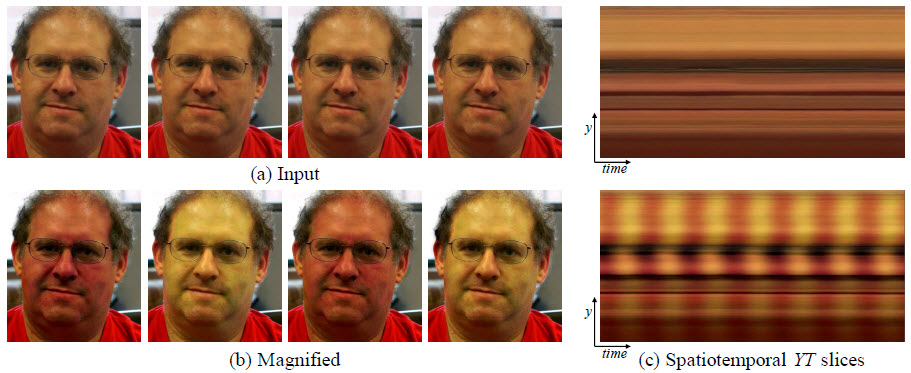
\includegraphics[width=0.7\textwidth, keepaspectratio=true]{mit-vidmag-teaser}
  \caption{The camera of the baby monitor}\cite{Wu12Eulerian}\cite{midvidmag-youtube}
  \label{fig:mit-vidmag}
\end{figure}

Refer to \cite{Poh2011Advancements}\cite{Wu12Eulerian}, we develop the baby monitor with computer vision to provide the following features:

\begin{compactitem}
\item motion detection
\end{compactitem}
\begin{compactitem}
\item pulse rate detection
\end{compactitem}
\begin{compactitem}
\item respiratory rate detection
\end{compactitem}
\begin{compactitem}
\item foreign object detection
\end{compactitem}
\begin{compactitem}
\item expression recognition
\end{compactitem}

\begin{figure}[b]
  \centering
	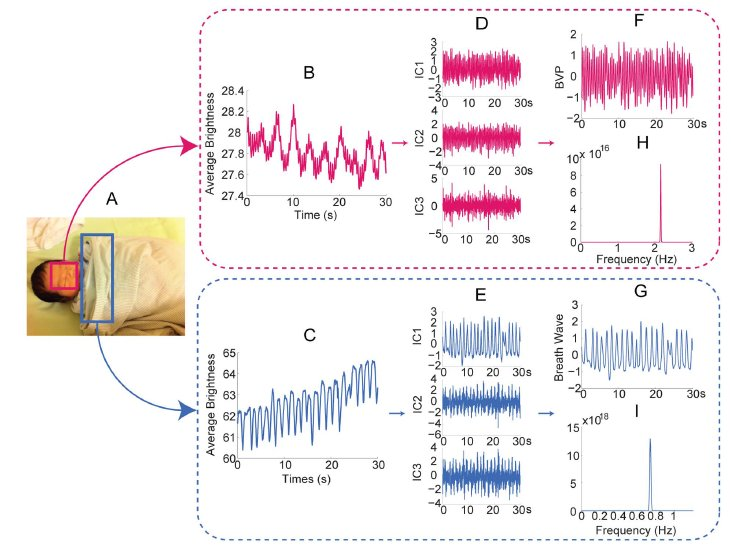
\includegraphics[width=0.8\textwidth, keepaspectratio=true]{baby-pr}
  \caption{baby pulse rate and respiratory rate}\cite{Hao-Yu-2013}
  \label{fig:baby-pr}
\end{figure}

%Figure~\ref{fig:paby-camera} shows a photograph of a gull.\cite{paby-monitor}
\clearpage
\section{Smart Glass}
We will focus on industrial and medical smart glass development with different light spectra.

\begin{figure}[ht]
  \centering
	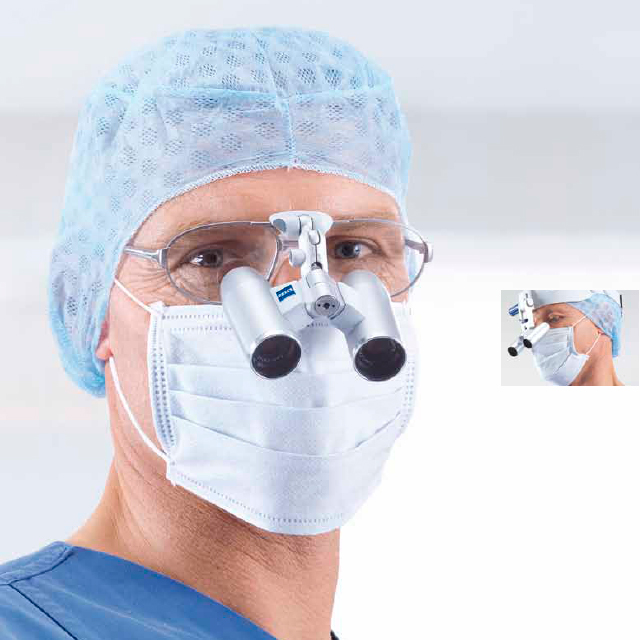
\includegraphics[width=0.7\textwidth, keepaspectratio=true]{medical-loupe-1}
  \caption{medical loupe}\cite{njnorth}
  \label{fig:medical-loupe}
\end{figure}

%Figure~\ref{fig:medical-loupe} shows a photograph of a gull.\cite{njnorth}

%----------------------------------------------------------------------------------------
%	REFERENCE LIST
%----------------------------------------------------------------------------------------
\clearpage
%\printbibliography
%\bibliography{abbr_long,pubext}
\bibliography{thomastsai.bib}{}
\bibliographystyle{ieeetr}
%\bibliographystyle{plain}

%\begin{thebibliography}{99} % Bibliography - this is intentionally simple in this template

%\bibitem[Figueredo and Wolf, 2009]{Figueredo:2009dg}
%Figueredo, A.~J. and Wolf, P. S.~A. (2009).
%\newblock Assortative pairing and life history strategy - a cross-cultural
%  study.
%\newblock {\em Human Nature}, 20:317--330.
 
%\end{thebibliography}

%----------------------------------------------------------------------------------------

\end{document}          
